\documentclass{ximera}
%\graphicspath{  %% When looking for images,
{./}            %% look here first,
{./pictures/}   %% then look for a pictures folder,
{../pictures/}  %% which may be a directory up.
{../../pictures/}  %% which may be a directory up.
{../../../pictures/}  %% which may be a directory up.
{../../../../pictures/}  %% which may be a directory up.
}

\usepackage{listings}
\usepackage{circuitikz}
\usepackage{xcolor}
\usepackage{amsmath,amsthm}
\usepackage{subcaption}
\usepackage{graphicx}
\usepackage{tikz}
\usepackage{tikz-3dplot}
\usepackage{amsfonts}
\usepackage{mdframed} % For framing content
\usepackage{tikz-cd}

  \renewcommand{\vector}[1]{\left\langle #1\right\rangle}
  \newcommand{\arrowvec}[1]{{\overset{\rightharpoonup}{#1}}}
  \newcommand{\ro}{\texttt{R}}%% row operation
  \newcommand{\dotp}{\bullet}%% dot product
  \renewcommand{\l}{\ell}
  \let\defaultAnswerFormat\answerFormatBoxed
  \usetikzlibrary{calc,bending}
  \tikzset{>=stealth}
  




%make a maroon color
\definecolor{maroon}{RGB}{128,0,0}
%make a dark blue color
\definecolor{darkblue}{RGB}{0,0,139}
%define the color fourier0 to be the maroon color
\definecolor{fourier0}{RGB}{128,0,0}
%define the color fourier1 to be the dark blue color
\definecolor{fourier1}{RGB}{0,0,139}
%define the color fourier 1t to be the light blue color
\definecolor{fourier1t}{RGB}{173,216,230}
%define the color fourier2 to be the dark green color
\definecolor{fourier2}{RGB}{0,100,0}
%define teh color fourier2t to be the light green color
\definecolor{fourier2t}{RGB}{144,238,144}
%define the color fourier3 to be the dark purple color
\definecolor{fourier3}{RGB}{128,0,128}
%define the color fourier3t to be the light purple color
\definecolor{fourier3t}{RGB}{221,160,221}
%define the color fourier0t to be the red color
\definecolor{fourier0t}{RGB}{255,0,0}
%define the color fourier4 to be the orange color
\definecolor{fourier4}{RGB}{255,165,0}
%define the color fourier4t to be the darker orange color
\definecolor{fourier4t}{RGB}{255,215,0}
%define the color fourier5 to be the yellow color
\definecolor{fourier5}{RGB}{255,255,0}
%define the color fourier5t to be the darker yellow color
\definecolor{fourier5t}{RGB}{255,255,100}
%define the color fourier6 to be the green color
\definecolor{fourier6}{RGB}{0,128,0}
%define the color fourier6t to be the darker green color
\definecolor{fourier6t}{RGB}{0,255,0}

%New commands for this doc for errors in copying
\newcommand{\eigenvar}{\lambda}
%\newcommand{\vect}[1]{\mathbf{#1}}
\renewcommand{\th}{^{\text{th}}}
\newcommand{\st}{^{\text{st}}}
\newcommand{\nd}{^{\text{nd}}}
\newcommand{\rd}{^{\text{rd}}}
\newcommand{\paren}[1]{\left(#1\right)}
\newcommand{\abs}[1]{\left|#1\right|}
\newcommand{\R}{\mathbb{R}}
\newcommand{\C}{\mathbb{C}}
\newcommand{\Hilb}{\mathbb{H}}
\newcommand{\qq}[1]{\text{#1}}
\newcommand{\Z}{\mathbb{Z}}
\newcommand{\N}{\mathbb{N}}
\newcommand{\q}[1]{\text{``#1''}}
%\newcommand{\mat}[1]{\begin{bmatrix}#1\end{bmatrix}}
\newcommand{\rref}{\text{reduced row echelon form}}
\newcommand{\ef}{\text{echelon form}}
\newcommand{\ohm}{\Omega}
\newcommand{\volt}{\text{V}}
\newcommand{\amp}{\text{A}}
\newcommand{\Seq}{\textbf{Seq}}
\newcommand{\Poly}{\textbf{P}}
\renewcommand{\quad}{\text{    }}
\newcommand{\roweq}{\simeq}
\newcommand{\rowop}{\simeq}
\newcommand{\rowswap}{\leftrightarrow}
\newcommand{\Mat}{\textbf{M}}
\newcommand{\Func}{\textbf{Func}}
\newcommand{\Hw}{\textbf{Hamming weight}}
\newcommand{\Hd}{\textbf{Hamming distance}}
\newcommand{\rank}{\text{rank}}
\newcommand{\longvect}[1]{\overrightarrow{#1}}
% Define the circled command
\newcommand{\circled}[1]{%
  \tikz[baseline=(char.base)]{
    \node[shape=circle,draw,inner sep=2pt,red,fill=red!20,text=black] (char) {#1};}%
}

% Define custom command \strikeh that just puts red text on the 2nd argument
\newcommand{\strikeh}[2]{\textcolor{red}{#2}}

% Define custom command \strikev that just puts red text on the 2nd argument
\newcommand{\strikev}[2]{\textcolor{red}{#2}}

%more new commands for this doc for errors in copying
\newcommand{\SI}{\text{SI}}
\newcommand{\kg}{\text{kg}}
\newcommand{\m}{\text{m}}
\newcommand{\s}{\text{s}}
\newcommand{\norm}[1]{\left\|#1\right\|}
\newcommand{\col}{\text{col}}
\newcommand{\sspan}{\text{span}}
\newcommand{\proj}{\text{proj}}
\newcommand{\set}[1]{\left\{#1\right\}}
\newcommand{\degC}{^\circ\text{C}}
\newcommand{\centroid}[1]{\overline{#1}}
\newcommand{\dotprod}{\boldsymbol{\cdot}}
%\newcommand{\coord}[1]{\begin{bmatrix}#1\end{bmatrix}}
\newcommand{\iprod}[1]{\langle #1 \rangle}
\newcommand{\adjoint}{^{*}}
\newcommand{\conjugate}[1]{\overline{#1}}
\newcommand{\eigenvarA}{\lambda}
\newcommand{\eigenvarB}{\mu}
\newcommand{\orth}{\perp}
\newcommand{\bigbracket}[1]{\left[#1\right]}
\newcommand{\textiff}{\text{ if and only if }}
\newcommand{\adj}{\text{adj}}
\newcommand{\ijth}{\emph{ij}^\text{th}}
\newcommand{\minor}[2]{M_{#2}}
\newcommand{\cofactor}{\text{C}}
\newcommand{\shift}{\textbf{shift}}
\newcommand{\startmat}[1]{
  \left[\begin{array}{#1}
}
\newcommand{\stopmat}{\end{array}\right]}
%a command to give a name to explorations and hints and theorems
\newcommand{\name}[1]{\begin{centering}\textbf{#1}\end{centering}}
\newcommand{\vect}[1]{\vec{#1}}
\newcommand{\dfn}[1]{\textbf{#1}}
\newcommand{\transpose}{\mathsf{T}}
\newcommand{\mtlb}[2][black]{\texttt{\textcolor{#1}{#2}}}
\newcommand{\RR}{\mathbb{R}} % Real numbers
\newcommand{\id}{\text{id}}
\graphicspath{  %% When looking for images,
{./}            %% look here first,
{./pictures/}   %% then look for a pictures folder,
{../pictures/}  %% which may be a directory up.
}
\usepackage{listings}
\lstdefinestyle{Matlab}{
  language=Matlab,
  basicstyle=\ttfamily,
  keywordstyle=\color{blue},
  commentstyle=\color{green},
  stringstyle=\color{red},
  morekeywords={matlab2tikz},
  morekeywords=[2]{1}, keywordstyle=[2]{\color{black}},
  identifierstyle=\color{black},
  stringstyle=\color{red},
  commentstyle=\color{green},
  showstringspaces=false,
  numbers=left,
  numberstyle={\tiny \color{black}},
  numbersep=9pt,
  emph=[1]{star_wars_ratings.mat, pivcol_new,B,A,t, reduced, v, tau},emphstyle=[1]\color{purple}, 
}
%make a maroon color
\definecolor{maroon}{RGB}{128,0,0}
%make a dark blue color
\definecolor{darkblue}{RGB}{0,0,139}
%define the color fourier0 to be the maroon color
\definecolor{fourier0}{RGB}{128,0,0}
%define the color fourier1 to be the dark blue color
\definecolor{fourier1}{RGB}{0,0,139}
%define the color fourier 1t to be the light blue color
\definecolor{fourier1t}{RGB}{173,216,230}
%define the color fourier2 to be the dark green color
\definecolor{fourier2}{RGB}{0,100,0}
%define teh color fourier2t to be the light green color
\definecolor{fourier2t}{RGB}{144,238,144}
%define the color fourier3 to be the dark purple color
\definecolor{fourier3}{RGB}{128,0,128}
%define the color fourier3t to be the light purple color
\definecolor{fourier3t}{RGB}{221,160,221}
%define the color fourier0t to be the red color
\definecolor{fourier0t}{RGB}{255,0,0}
%define the color fourier4 to be the orange color
\definecolor{fourier4}{RGB}{255,165,0}
%define the color fourier4t to be the darker orange color
\definecolor{fourier4t}{RGB}{255,215,0}
%define the color fourier5 to be the yellow color
\definecolor{fourier5}{RGB}{255,255,0}
%define the color fourier5t to be the darker yellow color
\definecolor{fourier5t}{RGB}{255,255,100}
%define the color fourier6 to be the green color
\definecolor{fourier6}{RGB}{0,128,0}
%define the color fourier6t to be the darker green color
\definecolor{fourier6t}{RGB}{0,255,0}

%New commands for this doc for errors in copying
\newcommand{\eigenvar}{\lambda}
\newcommand{\vect}[1]{\mathbf{#1}}
\renewcommand{\th}{^{\text{th}}}
\newcommand{\st}{^{\text{st}}}
\newcommand{\nd}{^{\text{nd}}}
\newcommand{\rd}{^{\text{rd}}}
\newcommand{\paren}[1]{\left(#1\right)}
\newcommand{\abs}[1]{\left|#1\right|}
\newcommand{\R}{\mathbb{R}}
\newcommand{\C}{\mathbb{C}}
\newcommand{\Hilb}{\mathbb{H}}
\newcommand{\qq}[1]{\text{#1}}
\newcommand{\Z}{\mathbb{Z}}
\newcommand{\N}{\mathbb{N}}
\newcommand{\q}[1]{\text{``#1''}}
\newcommand{\mat}[1]{\begin{bmatrix}#1\end{bmatrix}}
\newcommand{\rref}{\text{reduced row echelon form}}
\newcommand{\ef}{\text{echelon form}}
\newcommand{\ohm}{\Omega}
\newcommand{\volt}{\text{V}}
\newcommand{\amp}{\text{A}}
\newcommand{\Seq}{\textbf{Seq}}
\newcommand{\Poly}{\textbf{P}}
\renewcommand{\quad}{\text{    }}
\newcommand{\roweq}{\simeq}
\newcommand{\rowop}{\simeq}
\newcommand{\rowswap}{\leftrightarrow}
\newcommand{\Mat}{\textbf{M}}
\newcommand{\Func}{\textbf{Func}}
\newcommand{\Hw}{\textbf{Hamming weight}}
\newcommand{\Hd}{\textbf{Hamming distance}}
\newcommand{\rank}{\text{rank}}
\newcommand{\longvect}[1]{\overrightarrow{#1}}
% Define the circled command
\newcommand{\circled}[1]{%
  \tikz[baseline=(char.base)]{
    \node[shape=circle,draw,inner sep=2pt,red,fill=red!20,text=black] (char) {#1};}%
}

%an environment of proof extending to proof of
\newenvironment{proofof}[1]{%
  \proof[\textbf{Proof #1}]%
}{%
  \endproof
}

% Define custom command \strikeh that just puts red text on the 2nd argument
\newcommand{\strikeh}[2]{\textcolor{red}{#2}}

% Define custom command \strikev that just puts red text on the 2nd argument
\newcommand{\strikev}[2]{\textcolor{red}{#2}}

%an environment for \mymatrix
% Define the mymatrix environment
\newenvironment{mymatrix}[1]
  {% Begin code
   \left[\begin{array}{#1}}
  {% End code
   \end{array}\right]}
%an environment for \absmatrix
% Define the absmatrix environment
\newenvironment{absmatrix}[1]
  {% Begin code
   \left|\begin{array}{#1}}
  {% End code
   \end{array}\right|}

% Define the custom environment enumialphparenastyle that for now just makes everything red
\newenvironment{enumialphparenastyle}
{% Begin code - executed at the start of the environment
  \color{red} % Set text color to red
}
{% End code - executed at the end of the environment
}

% Define the custom environment mysmallmatrix
\newenvironment{mysmallmatrix}
{% Begin code - executed at the start of the environment
  \left[\begin{smallmatrix}
}
{% End code - executed at the end of the environment
  \end{smallmatrix}\right]
}

%define a new "ex" environment that is the same as the "exercise" environment
\newenvironment{ex}{\begin{exercise}}{\end{exercise}}
%define a new "sol" environment that is the same as the "solution" environment
\newenvironment{sol}{\begin{solution}}{\end{solution}}

%more new commands for this doc for errors in copying
\newcommand{\SI}{\text{SI}}
\newcommand{\kg}{\text{kg}}
\newcommand{\m}{\text{m}}
\newcommand{\s}{\text{s}}
\newcommand{\norm}[1]{\left\|#1\right\|}
\newcommand{\col}{\text{col}}
\newcommand{\sspan}{\text{span}}
\newcommand{\proj}{\text{proj}}
\newcommand{\set}[1]{\left\{#1\right\}}
\newcommand{\degC}{^\circ\text{C}}
\newcommand{\centroid}[1]{\overline{#1}}
\newcommand{\dotprod}{\boldsymbol{\cdot}}
\newcommand{\coord}[1]{\begin{bmatrix}#1\end{bmatrix}}
\newcommand{\iprod}[1]{\langle #1 \rangle}
\newcommand{\adjoint}{^{*}}
\newcommand{\conjugate}[1]{\overline{#1}}
\newcommand{\eigenvarA}{\lambda}
\newcommand{\eigenvarB}{\mu}
\newcommand{\orth}{\perp}
\newcommand{\bigbracket}[1]{\left[#1\right]}
\newcommand{\textiff}{\text{ if and only if }}
\newcommand{\adj}{\text{adj}}
\newcommand{\ijth}{\emph{ij}^\text{th}}
\newcommand{\minor}[2]{M_{#2}}
\newcommand{\cofactor}{\text{C}}
\newcommand{\shift}{\textbf{shift}}


%Some boiler plate for putting matlab in 
%Write A as a matrix in MATLAB in a lstlisting environment
%\begin{lstlisting}[style=Matlab]
%    A = [1 0 3; 0 1 5; 1 1 8]
%    reduced=rref(A)
%\end{lstlisting}
\author{Zack Reed}
%borrowed from selinger linear algebra
\title{Discussion}
\begin{document}
\begin{abstract}

    In this introductory discussion, you will as a class explore the basics of vectors both geometrically and in different contexts.

\end{abstract}
\maketitle


\section*{Discussion Introduction}

  In the reading this week, you'll learn about how vectors can be used to represent data, physical concepts, lists of numbers, and really anything for which adding and multiplying by numbers makes sense. 
  
  A main theme of the course is going to be the interplay between geometry and application. Specifically, we'll see time and again that rules for vector and matrix manipulation established in geometry tell us how best to apply vectors and matrices to solve problems in other areas. This week's discussion will set up this theme by having you explore the geometry of vectors by playing and reflecting on the game Vector Unknown, and then using Vectors to see how we can tell machines to make sense of words and sentences in a way that is similar to how we make sense of them.

\section*{An Intro to Linear Combinations}

  The ``linear" in  ``Linear Algebra'' is largely captured by two key operations: addition and multiplication by scalars. We can do both at the same time in what's called a \emph{linear combination}. Linear combinations are the bread and butter of many important calculations in Linear Algebra. 

  If we have two vectors $\vec{v}$ and $\vec{w}$, and two scalars (e.g. real numbers) $a$ and $b$ then a linear combination of $\vec{v}$ and $\vec{w}$ is a new vector of the form $a\vec{v} + b\vec{w}$.

  For instance, if $\vec{v}=\begin{bmatrix}1\\-2\end{bmatrix}$, $\vec{u}= \begin{bmatrix}3\\4\end{bmatrix}$, and $\vec{w}=\begin{bmatrix}1\\-3\end{bmatrix}$, then $\vec{v} + +2\vec{u}+3\vec{w} = \begin{bmatrix}1\\-2\end{bmatrix} + 2\begin{bmatrix}3\\4\end{bmatrix} + 3\begin{bmatrix}1\\-3\end{bmatrix} = \begin{bmatrix}1\\-2\end{bmatrix} + \begin{bmatrix}6\\8\end{bmatrix} + \begin{bmatrix}3\\-9\end{bmatrix} = \begin{bmatrix}10\\-3\end{bmatrix}$.

  We geometrically find the result of this linear combination as is visualized in the GeoGebra applet below. We follow the first vector $\vec{v}$, then add the second vector $2\vec{u}$ to the end (the ``tip'' or the ``head''), then add the third vector $3\vec{w}$ to the end of that. The final vector is the one that starts at the origin and ends at the tip of the last vector we added.

  Put the vectors $\vec{v}$, $\vec{u}$, and $\vec{w}$ and the scalars $1$, $2$, and $3$ into the GeoGebra applet below to see the result of the linear combination $1\vec{v} + 2\vec{u} + 3\vec{w}$.

  \begin{center}
    \geogebra{serypqvd}{800}{600}
  \end{center}

  Here, we follow the first vector $\vec{v_1}$, then follow the two orange vectors after $\vec{v_1}$, and the result is the same as the blue vector $\vec{S}$, which as we computed is $\begin{bmatrix}10\\-3\end{bmatrix}$.

  \subsection*{Vector Unknown: Exploring Vectors and Linear Combinations}

  In the game Vector Unknown, you'll control a bunny rabbit who wants to find food, keys, and other objects within a field. You'll be given the target vector, where the object is located, and you'll need to direct the bunny to the target vector by taking linear combinations of provided vectors. 

  Here's a brief video walking through the basic controls of the game:

  \begin{center}
    %\youtube{1JW3xJ1QZ1A}
    Some YouTube Video
  \end{center}

  \subsubsection*{Task One}

  Play through the "Easy" difficulty and answer the following questions:
  \begin{enumerate}

    \item If your first attempt went off course, what did you do to correct and bring the bunny back to the target vector?
    \item In number 7, you were told that all targets lay along the line $t\vec{v}+\vec{w}$, where $\vec{v}$ and $\vec{w}$ were given. If you were then given a new target that lay off of this line, would you be able to reach it by taking linear combinations of $\vec{v}$ and $\vec{w}$? If so, how would you reach it? If not, why?

  \end{enumerate}

  Now play through the "Medium" difficulty and answer the following questions:

  \begin{enumerate}

    \item In number 3, you needed to find two keys and then find the lock. If you were given just one vector to work with, could you have accomplished the task? If so, how? If not, why?
    \item While there are four vectors available to you in number 3, what is the minimum number of vectors you need to reach find the keys and reach the lock? Why?
    \item In number 4, all of the food is located along a line through the origin. Said differently, all of the food is located in the span of a single vector. If a new piece of food was placed off of this line, what new vectors would not allow you to reach the food? What new vectors \emph{would} allow you to reach the food? Why?

  \end{enumerate}

\section*{Movie Ratings: Making Sense of Data as Vectors}

  We're going to look into our first application of vectors! We'll start with a context in which some of the early concepts we care about (e.g. vector arithmetic, distances between vectors, vector norms) are all raedily accessible and allow us some initial insight into how we help computers make sense of the real world through nubmers. 

  We'll be using MATLAB to organize and do some calculations on and visualizations of the data, and then we'll use the results of the MATLAB calculations to make sense of the the data. 

  \begin{hint} 

    For a primer on installing MATLAB with all of the required toolboxes, setting up the helper files for the class into the right folders, and getting started with a few calculations, check out the video below:

    \begin{center}
      %\youtube{1JW3xJ1QZ1A}
      Some YouTube Video
    \end{center}

  \end{hint}

  \subsection*{Making Sense of Clusters in Data}

  Looking back at the fruit classification example from the early sections of the book, we already examined the potential insights gained from clusters of vectors where the dimensions of the vectors were measurements of fruit. 

  \begin{example}
    In this hypothetical example, where we took the measurements of pear and apple weights, max circumferences, and stem lengths, a data scientist might hope that there's an easy way to geometrically separate all of the apple vectors from pear vectors in a given data set. They'd then use that geometry to predict whether a new fruit is an apple or a pear based on its measurement. 


    \begin{center}
        %\pdfOnly{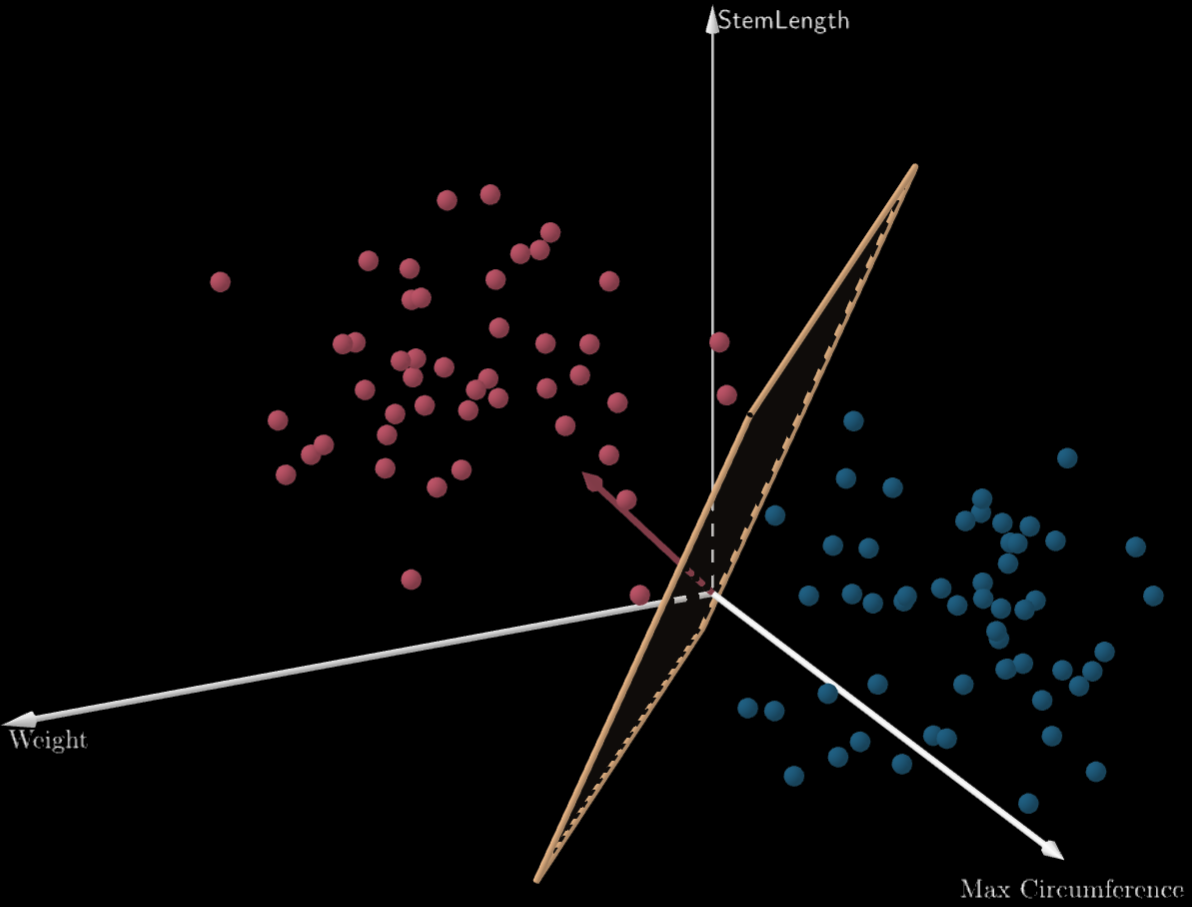
\includegraphics[width=.75\textwidth]{apple-pear.png}\\
       % $$\vec{F}\text{ is within the Apple cluster, and is thus an apple rather than a pear.}$$}
        \geogebra{qnghrmdg}{800}{600} %%https://www.geogebra.org/m/qnghrmdg
    \end{center}

    In this very idealistic example, vectors that are closer to the apple cluster are more likely to be apples, and vectors that are closer to the pear cluster are more likely to be pears. Hit the "New Fruit" button a few times to see how this plays out.

    We'll do a very similar thing now with movie ratings, but we'll use the distances between vectors as a way to compare how similar two raters are to each other.

    
\end{example}

  \subsection*{Movie Ratings: Getting Started}
  %https://grouplens.org/datasets/movielens/
  We're going to draw some idealized data from a larger data set of people's preferences for certain movies. We'll be looking at a very idealistic subset of the data, one where every rater has rated every movie on the list. We'll deal with a slightly more complicated example later for the course projects. 

  The full data set contains around 1 million ratings of 3952 movies by 6040 users. One issue with the data set is that, as one might expect, not every rater has rated every movie, so that introduces some complexities that data scientists spend lots of time dealing with. We're just going to look at a simpler subset of the data where 125 users have rated 20 movies.

  For now, we'll be looking at people's ratings (1:bad to 5:good) for the following 20 movies:

  \begin{itemize}

    \item E.T. the Extra-Terrestrial (1982) 
    \item Star Wars Episode IV - A New Hope (1977) 
    \item Star Wars Episode V - The Empire Strikes Back (1980) 
    \item Star Wars Episode VI - Return of the Jedi (1983) 
    \item Jurassic Park (1993) 
    \item Saving Private Ryan (1998) 
    \item Terminator 2 (1991)
    \item Matrix, The (1999) 
    \item Back to the Future (1985) 
    \item Silence of the Lambs, The (1991) 
    \item Star Wars Episode I - The Phantom Menace (1999) 
    \item Raiders of the Lost Ark (1981) 
    \item Fargo (1996) 
    \item Sixth Sense, The (1999) 
    \item Braveheart (1995) 
    \item Shakespeare in Love (1998) 
    \item Princess Bride, The (1987) 
    \item Schindler's List (1993) 
    \item Shawshank Redemption, The (1994) 
    \item Groundhog Day (1993) 

  \end{itemize}

  First, to get an idea of how we'll approach the data, we'll look at the ratings of 3 movies, the original Star Wars Trilogy, which lets us visualize the data.

  To get things started, open up a MATLAB live script and load star\_wars\_ratings.mat.

  \begin{hint}{MATLAB Code}
    %\revealbutton{Click to see MATLAB code}
        %Write A as a matrix in MATLAB in a lstlisting environment
        %\begin{pdfOnly}
          %\begin{lstlisting}[style=Matlab]
          \begin{verbatim}
              load star_wars_ratings.mat
          \end{verbatim}
          %\end{lstlisting}
        %\end{pdfOnly}
  \end{hint}

  Let's visualize the differences and similarities in these 125 users' ratings of the Star Wars Trilogy. Either plot the points on your own, or use the course helper function ``plot\_star\_wars'', being sure to input the vector list ``star\_wars\_ratings'' as an argument.

  \begin{hint}{MATLAB Code}
    %\begin{pdfOnly}
        %\begin{lstlisting}[style=Matlab]
        \begin{verbatim}
            linalg.plot_star_wars(star_wars_ratings)
        \end{verbatim}
        %\end{lstlisting}
      %\end{pdfOnly}
  \end{hint}

  Your plot should look something like the Figure below, and you should be able to click and drag within the figure to rotate the plot and see the data from different angles.

  \begin{center}
    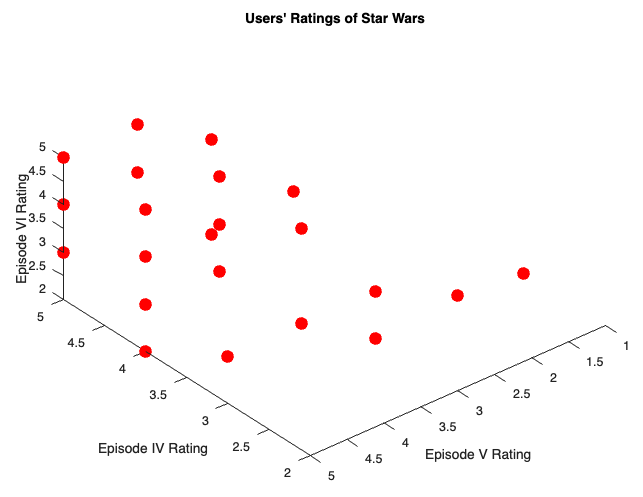
\includegraphics[width=.75\textwidth]{star_wars_ratings.png}
  \end{center}

  Unsurprisingly, many users rated the original Star Wars Trilogy highly, as most of the points are towards the upper left of the plot (where the ratings are higher). This doesn't account for how many users fall in each category, however, as there's no indication of how  many users fall on each dot. 

  Let's warm up by comparing the number of users located at [5,5,5] to the number of users located at [3,1,2] (the user who had the lowest ratings of the movies).

  This will be an opportunity to learn a few useful MATLAB commands that will be used throughout the course. The first is the ``norm'' function, which calculates the norm of a vector, which we learned about this module.

  Let's try it out to find the norms of our two vectors in question. 

  \begin{hint}{MATLAB Code}
    %\begin{pdfOnly}
    %\begin{lstlisting}[style=Matlab]
    \begin{verbatim}
        best=[5,5,5];
        worst=[3,1,2];
        best_norm=norm(best);
        worst_norm=norm(worst);
    \end{verbatim}
    %\end{lstlisting}
    %\begin{pdfOnly}
  \end{hint}

  \begin{example}

    The norm of the vector $[5,5,5]$ is $\sqrt{5^2+5^2+5^2}=\sqrt{75}\approx \answer{8.66}$, and the norm of the vector $[3,1,2]$ is $\sqrt{3^2+1^2+2^2}=\sqrt{14}\approx \answer{3.74}$.

  \end{example}

  We're going to use these norms to see how many users rated the movies in the best and worst categories. This will use want's called a "for loop" in MATLAB, which is a way to do lots of calculations at once without the computer having to be told to do each one individually.

  \begin{example}
  
  For instance, if you wanted to quickly calculate the square of each nubmer from 1 to 10, you could use the following code:
  \begin{verbatim}

        for i=1:10
            i_squared=i^2
        end

  \end{verbatim}

    With just three lines of code, you quickly get the computer to tell you all of the squares of the first 10 numbers. We'll be using for loops quite a bit in this course, as ways to quickly do lots of calculations. 

  \end{example}

    We'll use a for loop to count how many users rated the movies in the best and worst categories. We'll loop through the whole list of users, calculating each norm along the way, and compare it to the norms of the best and worst ratings. For the comparison, we need to use what's called an "if statement" in MATLAB, which is a way to tell the computer to do something only if a certain condition is met.

    \begin{example}

      For instance, if we wanted to check which number(s) from 1 to 10 squared to 25, we could use an "if" statement in the following way:
%\begin{pdfOnly}
      %\begin{lstlisting}[style=Matlab]
      \begin{verbatim}
          for i=1:10
              i_squared=i^2;
              if i_squared==25
                  i
              end
          end
      \end{verbatim}
      %\end{lstlisting}
   % \end{pdfOnly}

      This code only outputs the number 5, as 5 is the only number from 1 to 10 that squares to 25. For each other "i" from 1 to 10, the computer first defined ``i\_squared'' as $i^2$, and then checked if $i^2$ was equal to 25. If it was, the computer outputted the value of $i$.

      Note that we had to use ``=='' instead of just ``='', since ``='' is used to assign values to variables in MATLAB, and ``=='' is used to check if two values are equal.

    \end{example}
    
    We're going to start two numbers, best\_count and worst\_count, at 0, and then we're going to loop through each user's ratings. 
    
    If the norm of the user's ratings is equal to the norm of the best ratings, we'll add one to best\_count. If the norm of the user's ratings is equal to the norm of the worst ratings, we'll add one to worst\_count.

    I'll get you started in the hint, you alter the code to do what we want. Paste your code into the discussion, and then also answer the following questions:

    \begin{enumerate}

      \item How many users rated the movies in the best category?
      \item How many users rated the movies in the worst category?
      \item Could we catch any users in either category that had different ratings from [5,5,5] or [3,1,2]? If so, what are the other possible ratings?
      
    \end{enumerate}

    \begin{hint}

      Remember that ``star\_wars\_ratings'' is a matrix of row vectors, and that matrices' dimensions are organized first by rows and then by columns. You can access the ith user's ratings with 
      %\begin{pdfOnly}
      %\begin{lstlisting}[style=Matlab]
      \begin{verbatim}
        star_wars_ratings(i,:)
      \end{verbatim}
      %\end{lstlisting}
    %\end{pdfOnly}
      
      which returns a vector of the form [rating\_1, rating\_2, rating\_3].

    \end{hint}

    \begin{hint}{MATLAB Code}
      %\begin{pdfOnly}
      %\begin{lstlisting}[style=Matlab]
      \begin{verbatim}
          best=[5,5,5];
          worst=[3,1,2];
          best_norm=norm(best);
          worst_norm=norm(worst);
          best_count=0;
          worst_count=0;
          for i=1:125
              %Check if the norm of the ith user's ratings is equal to the norm of the best ratings
              if %your code here
                  best_count=best_count+1;
              end
              %Check if the norm of the ith user's ratings is equal to the norm of the worst ratings
              if %your code here
                  worst_count=worst_count+1;
              end
          end
      \end{verbatim}
      %\end{lstlisting}
   % \end{pdfOnly}
    \end{hint}

    \subsection*{Task Two: Predicting Recommendations}

    We don't just use data to make observations, but also to find patterns that allow us to predict unknown events. The strategy is to use our observed data to find patterns, and then to use those patterns for prediction. In this case, we're going to see if the users' ratings of the Star Wars Trilogy can predict their ratings of ``Star Wars Episode I - The Phantom Menace (1999)''. 

    Let's use you and two of your friends or family members as test cases in the following way: 
    
    \begin{enumerate}
    
      \item  Rate all four movies from 1 to 5 and ask your friends to do the same. 
      \item Find the norms of your ratings and your friends' ratings.
      \item Find the users in the data set whose ratings of the \emph{Original Trilogy} are closest to yours, and then do the same for your friends' ratings.
      \item Load phantom\_menace\_ratings.mat to average the closest users' ratings of ``Star Wars Episode I - The Phantom Menace (1999)''. The indices of phantom\_menace\_ratings correspond to the indices of the users in the data set, so you can use the same indices you found in the previous step to find the ratings of the closest users.
      \item Share your results with the class, and see if you can explain why the predictions were or were not accurate, and what we might do to improve them.
      \item Reflect on the following question: Is just using the norm of the ratings a good way to predict how users will rate movies? What users' ratings might we unintentionally catch in our predictions, and how might we avoid this?
    \end{enumerate}

    \begin{hint}

      You'll want to isolate only the users who rated the Original Trilogy like you did, and then average their ratings of ``Star Wars Episode I - The Phantom Menace (1999)''. To just isolate the closest users and get their new rating, all you need are the index values of the users. So within the loop to find the closest users, you can just append each new index to a previous list of indices, and then use that list to find the new ratings.

      For instance, if you wanted to find which elements of the list [1, 2, 3, 2, 3, 5, 1, 2] square to 4, you could use the following code:
      %\begin{pdfOnly}
      %\begin{lstlisting}[style=Matlab]
      \begin{verbatim}
        indices=[];
        list=[1, 2, 3, 2, 3, 5, 1, 2];
        for i=1:8
            number=list(i);
            squared=number^2;
            if squared==4
                indices=[indices,i];
            end
        end
      \end{verbatim}
      %\end{lstlisting}
   % \end{pdfOnly}
      
      This will start with an empty list of indices, and then add the index of each element of the list that squares to 4 to the list of indices. The line ``indices=[indices,i]'' appends the index of the element to the list of indices.

      Then, you can get a smaller list of the elements that squared to 4 by using the list of indices:
      %\begin{pdfOnly}
      %\begin{lstlisting}[style=Matlab]
      \begin{verbatim}
        new_list=list(indices)
      \end{verbatim}
        
      %\end{lstlisting}
      %\end{pdfOnly}


      This will return the list [2, 2, 2], as the 2nd, 4th, and 8th elements of the original list squared to 4.

      Finally, you'll also want to average the ratings of the closest users. You can take the average of a list of numbers in MATLAB with the ``mean'' function. For instance, if you wanted to find the average of the list [1, 2, 3, 4, 5], you could use the following code:

      %\begin{pdfOnly}
      %\begin{lstlisting}[style=Matlab]
      \begin{verbatim}
        list=[1, 2, 3, 4, 5];
        average=mean(list)        
      \end{verbatim}

      %\end{lstlisting}

    %\end{pdfOnly}

      This will return the value 3, as the average of 1, 2, 3, 4, and 5 is 3.

    \end{hint}


      
      
  \subsection*{Task Three: Scaling Up}

    To get more nuanced data, we don't only want to compare the ratings of similar movies like the Star Wars Trilogy, but ideally we'd like to predict users' ratings of varoius movies from all kinds of genres. We'll still stick to ideal data and the somewhat naive comparison of distance, but we'll get a better feel for how we might scale up our analysis.

    We're going to take all 125 users' ratings of the first 19 movies, and then see how closely we can use their ratings to make predictions for three test users' ratings of the 20th movie, ``Groundhog Day (1993)''. This is common when training more complicated methods of computer prediction, to split the data into "training" and "testing" data so that the predictive power of our models can be assessed.

    As we saw in Task Two, we should be more nuanced in our analysis than just using the norms of vectors for comparison. Instead, we'll find the users whose vectors are closest to the test users' vectors, and then average their ratings of the 20th movie to make our prediction. The importance of using distance instead of just norm comparison is that we're minimizing the difference between the test users and potentially close users, so that we only use the vectors that lie within very similar regions of our 19-dimensional space.

    Do the following to complete the activity:

    \begin{enumerate}

      \item Load the data set ``training\_ratings.mat'' into MATLAB.
      \item Load the test users' ratings of the first 19 movies from ``test\_ratings.mat''.
      \item Find the training users whose ratings of the first 19 movies are less than a distance of 1, 2, and 3 from the test users' ratings. If there are none, find the closest training user possible.
      \item Load the ratings of the 20th movie, ``Groundhog Day (1993)'', from ``groundhog\_day\_train.mat'' and ``groundhog\_day\_test.mat''.
      \item Average the closest users' ratings of the 20th movie, ``Groundhog Day (1993)'' and compare the average to the test users' ratings.
      \item Share your results with the class. Think about what factors might be obscuring predictability by also getting a feel for the test users as well. For isntance, are they harsh raters? Easy raters? What other factors might be at play in the data that we're not considering?
    \end{enumerate}

    \begin{hint}

      If you need to find the user with the single minimum distance from a test user, there are a few ways to do this, but one of the easiest ways is to first make a vector of the distances between the test user and all of the training users, and then find the index of the minimum value of that vector using the ``min'' function.

      As an example, if you wanted to find the index of the number with the minimum square value from the list [3, 3, 1, 2, 3, 4, 5, 2], you could do the following:
      %\begin{pdfOnly}
      %\begin{lstlisting}[style=Matlab]
      \begin{verbatim}
        list=[3, 3, 1, 2, 3, 4, 5, 2];
        squared_list=[]
        for i=1:8
            number=list(i);
            squared=number^2;
            squared_list=[squared_list,squared];
        end
        [square, idx]=min(squared_list)
      \end{verbatim}
      %\end{lstlisting}
    %\end{pdfOnly}

      The syntax [square,idx] means that the ``min'' function returns two numbers, first the minimum value and then second the index of that value in the original list. It should return square=1 and idx=3, as the 3rd element of the original list squared to 1.

    \end{hint}

\end{document}